\documentclass[9pt,twocolumn,twoside]{article}

\usepackage[letterpaper,margin=1.6cm,columnsep=0.7cm]{geometry}
\usepackage{graphicx}
\usepackage{amsmath}
\usepackage{times}
\usepackage[T1]{fontenc}
\usepackage{microtype}
\usepackage{caption}
\usepackage{authblk}
\usepackage[hidelinks]{hyperref}
\usepackage{xcolor}
\usepackage{titlesec}
\usepackage{abstract}
\usepackage{booktabs}
\usepackage{array}

\captionsetup{font=small,labelfont=bf,labelsep=period}
\titleformat{\section}{\normalfont\bfseries\large}{\thesection}{0.6em}{}
\titleformat{\subsection}{\normalfont\bfseries}{\thesubsection}{0.6em}{}
\titlespacing{\section}{0pt}{1.4ex}{0.6ex}
\titlespacing{\subsection}{0pt}{1.0ex}{0.4ex}
\setlength{\parindent}{1.1em}
\renewcommand{\abstractnamefont}{\normalfont\bfseries}
\renewcommand{\abstracttextfont}{\normalfont\small}

\title{\vspace{-1.2em}\bfseries Enactome: a connectome-constrained simulation platform reveals
dimensionality compression and aversion bias in the Drosophila lateral horn}

\author[1]{Mehmet Kerem Turkcan}
\affil[1]{Associate Research Scientist, Columbia University, USA. \texttt{mkt2126@columbia.edu}}
\date{}

\begin{document}
\twocolumn[
\maketitle
\begin{onecolabstract}
\noindent
The reconstruction of complete insect connectomes provides synaptic wiring diagrams whose
computational function remains to be established. We present Enactome, a simulation platform that
loads the Brain and Nerve Cord (BANC) connectome of 158,262 neurons and 3,990,039 synapses, assigns
each connection a sign from its presynaptic transmitter, and evaluates circuit function through rate,
integrate-and-fire, and Hodgkin-Huxley neuron models on shared central processing and graphics
processing backends. Applying the platform to the olfactory pathway, we find that the lateral horn
reduces the dimensionality of the odor representation by a factor of 1.60 relative to its projection
neuron input and raises the mean correlation between odor representations by 0.15. Both effects
exceed degree-preserving shuffles of the same wiring (z = 6.2 and z = 16.4), which establishes them
as consequences of the specific glomerular projection pattern. The lateral horn output is biased
toward aversion, with aversive-tuned output neurons outnumbering appetitive-tuned neurons by a ratio
of 2.24 to 1, and graded silencing of these neurons reduces the innate valence readout
monotonically. The platform reproduces additional published observations across the mushroom body,
central complex, visual system, neuromodulatory systems, and whole-brain excitation-inhibition
balance through a registry of 35 quantitative experiments, each recreating a specific finding by
simulation of the same connectome. A gene-to-cell-type layer built from single-cell expression and
human-ortholog data links circuit elements to human disease and identifies the endogenous targets of
optogenetic manipulation. Applied to the central-complex heading circuit, the platform recovers the
ring-attractor architecture and its ring topology from the wiring alone, but shows that a
connectome-constrained rate model settles into a small number of discrete heading states rather than
a continuous representation, delimiting what the wiring alone determines. Enactome converts a static
wiring diagram into a testable model of circuit computation.
\vspace{1.0em}
\end{onecolabstract}
]

\section{Introduction}
Electron-microscopy reconstruction has produced synaptic connectomes for the fruit fly at the scale
of the entire central brain and ventral nerve cord \cite{dorkenwald2024,schlegel2024}. These datasets
enumerate neurons and their synaptic contacts, yet a wiring diagram alone does not specify what a
circuit computes. Bridging structure and function requires models that combine the measured
connectivity with neuron dynamics and that can be interrogated in the same way an experimentalist
interrogates a preparation, through stimulation, silencing, and measurement of a defined output.

Earlier platforms established interactive access to fly connectome data and the emulation of
selected circuits. The Fruit Fly Brain Observatory provided a repository and natural-language and
graphical interfaces for querying and executing circuit models \cite{ukani2019}, and FlyBrainLab
provided an integrated computing environment linking connectome data to executable circuits
\cite{lazar2021}. Enactome builds on this lineage by pairing a whole-connectome engine with several
levels of neuron abstraction and a registry of reproducible experiments that recreate published
findings, on an organism-general codebase for which the adult fruit fly is the current incarnation.

Existing connectome analyses often examine one circuit with a bespoke model. A general platform that
loads a whole connectome, supports several levels of neuron abstraction, and records reproducible
experiments would allow findings in one circuit to be evaluated against the constraints of the whole
brain. Here we describe Enactome, which provides this capability, and we use it to characterize the
computation performed by the lateral horn, a higher olfactory center that mediates innate responses
to odor.

The lateral horn receives projection-neuron input from the antennal lobe and has been associated
with genetically hardwired valence \cite{frechter2019,dolan2019,daschakraborty2022}. Its
transformation of the olfactory code has not been quantified against a wiring-preserving statistical
baseline. We report that the lateral horn compresses and decorrelates the odor representation and
that its output is quantitatively biased toward aversion, and we show that these properties depend on
the specific connectivity rather than on the coarse degree distribution of the network.

\begin{figure*}[t]
\centering
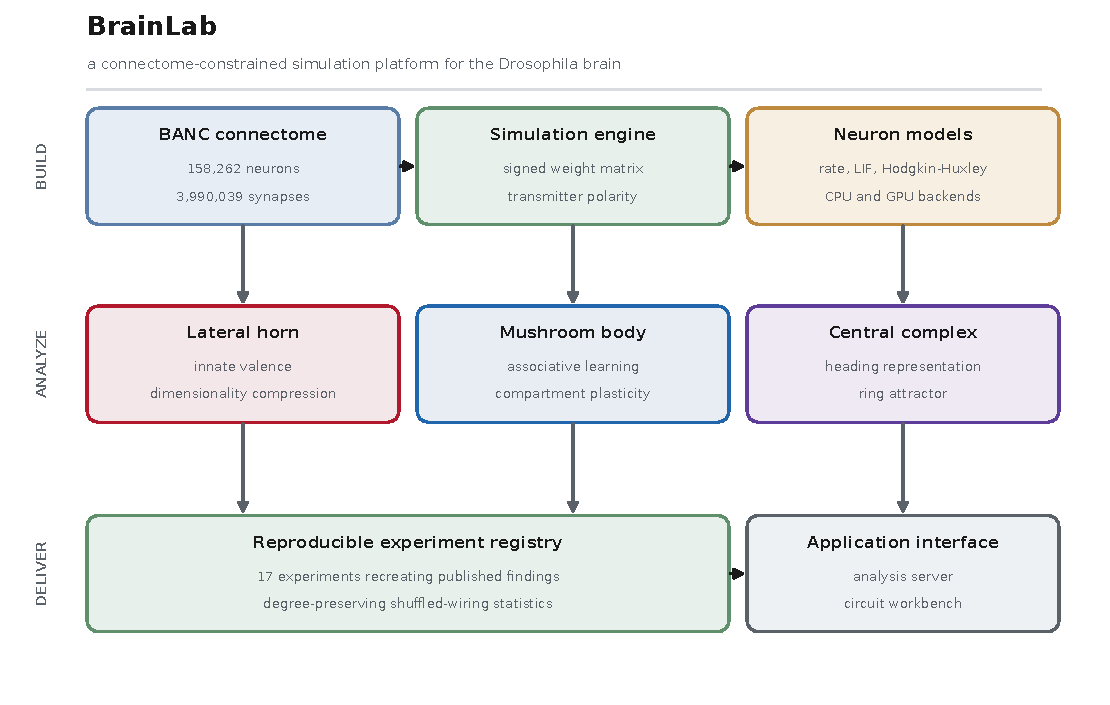
\includegraphics[width=0.94\textwidth]{fig1_platform.pdf}
\caption{\textbf{Architecture of the Enactome platform.} The BANC connectome is loaded into a
simulation engine that assigns each synapse a sign from the presynaptic transmitter identity. A
multi-level neuron backend evaluates the resulting signed network with rate, integrate-and-fire, and
Hodgkin-Huxley models on central processing and graphics processing backends. Three olfactory and
navigational subsystems are analyzed through the same engine, and results are recorded in a registry
of reproducible experiments that is exposed through an analysis server and a circuit workbench.}
\label{fig:platform}
\end{figure*}

\section{Results}

\subsection{A connectome-constrained simulation platform}
Enactome loads the BANC connectome and represents it as a signed weighted adjacency matrix. Each
directed synapse carries a weight equal to its reconstructed synapse count and a sign determined by
the predicted transmitter of the presynaptic neuron, with acetylcholine treated as excitatory and
gamma-aminobutyric acid and glutamate treated as inhibitory in the fly central brain. The platform
evaluates this network through three neuron models that share a common numerical backend
(Fig.~\ref{fig:platform}). A rate model integrates a leaky firing-rate equation and scales to the
full network of 158,262 neurons. An integrate-and-fire model uses membrane parameters calibrated to
fly central neurons \cite{shiu2024,kakaria2017}, with a resting and reset potential of -52~mV, a
threshold of -45~mV, a membrane resistance of 10~M$\Omega$, a membrane time constant of 20~ms, and a
synaptic weight of 0.275~mV per synapse, which places the threshold at approximately 25 coincident
synaptic events. A Hodgkin-Huxley model \cite{hodgkin1952} provides biophysical detail for single
neurons. Both central processing and graphics processing backends produce identical results.

Neuromodulation is represented as a receptor-dependent change in the gain and bias of the affected
neurons \cite{nadim2014}, with dopamine, octopamine, and acetylcholine increasing gain and serotonin
decreasing it. The mushroom body implements a dopamine-gated plasticity rule in which coincident
Kenyon-cell activity and compartmental dopaminergic activity depress the Kenyon-cell to output-neuron
synapses within that compartment \cite{aso2014}.

\subsection{The lateral horn compresses and decorrelates the odor representation}
We traced the pathway from olfactory receptor neurons through uniglomerular projection neurons to
lateral horn output neurons (Fig.~\ref{fig:lh}a). We presented a panel of single-glomerulus odor
inputs and measured the dimensionality of the population representation at the projection-neuron and
output-neuron layers using the participation ratio. The lateral horn representation had a lower
dimensionality than its input by a factor of 1.60, despite the output layer containing more neurons
(1,079) than the projection-neuron layer (451) (Fig.~\ref{fig:lh}b). Over the same odor panel, the
mean pairwise correlation between odor representations increased by 0.15 from the projection-neuron
layer to the lateral horn (Fig.~\ref{fig:lh}c).

To determine whether these transformations reflect the specific glomerular wiring or only the coarse
connection statistics, we compared each measurement against a null distribution generated by randomly
permuting the nonzero synaptic weights among the existing projection-neuron to output-neuron
connections. This procedure preserves the number of connections and the distribution of synaptic
weights while destroying the specific pairing that carries glomerular identity. The observed
compression exceeded the null by 6.2 standard deviations, and the observed rise in correlation
exceeded the null by 16.4 standard deviations (permutation p = 0.002 for each, 500 shuffles). The
compression and decorrelation of the odor code are therefore properties of the specific connectivity.

\subsection{Lateral horn output is biased toward aversion}
We assigned each output neuron a valence index from the hardwired valence of the glomeruli that
supply its projection-neuron input. Aversive-tuned output neurons outnumbered appetitive-tuned output
neurons by a ratio of 2.24 to 1, with 285 aversive and 127 appetitive neurons among the 1,079 output
neurons (Fig.~\ref{fig:lh}d). Graded silencing of output neurons reduced the innate valence readout
monotonically, from a value of 81 in the intact circuit to zero when all output neurons were silenced
(Fig.~\ref{fig:lh}e). Lateral horn local neurons, which are predominantly GABAergic and
glutamatergic, provide feedforward inhibition onto the output neurons: removing their synaptic input
raised the mean net input onto output neurons from 6.7 to 11.8, consistent with a disinhibitory
role.

\begin{figure*}[t]
\centering
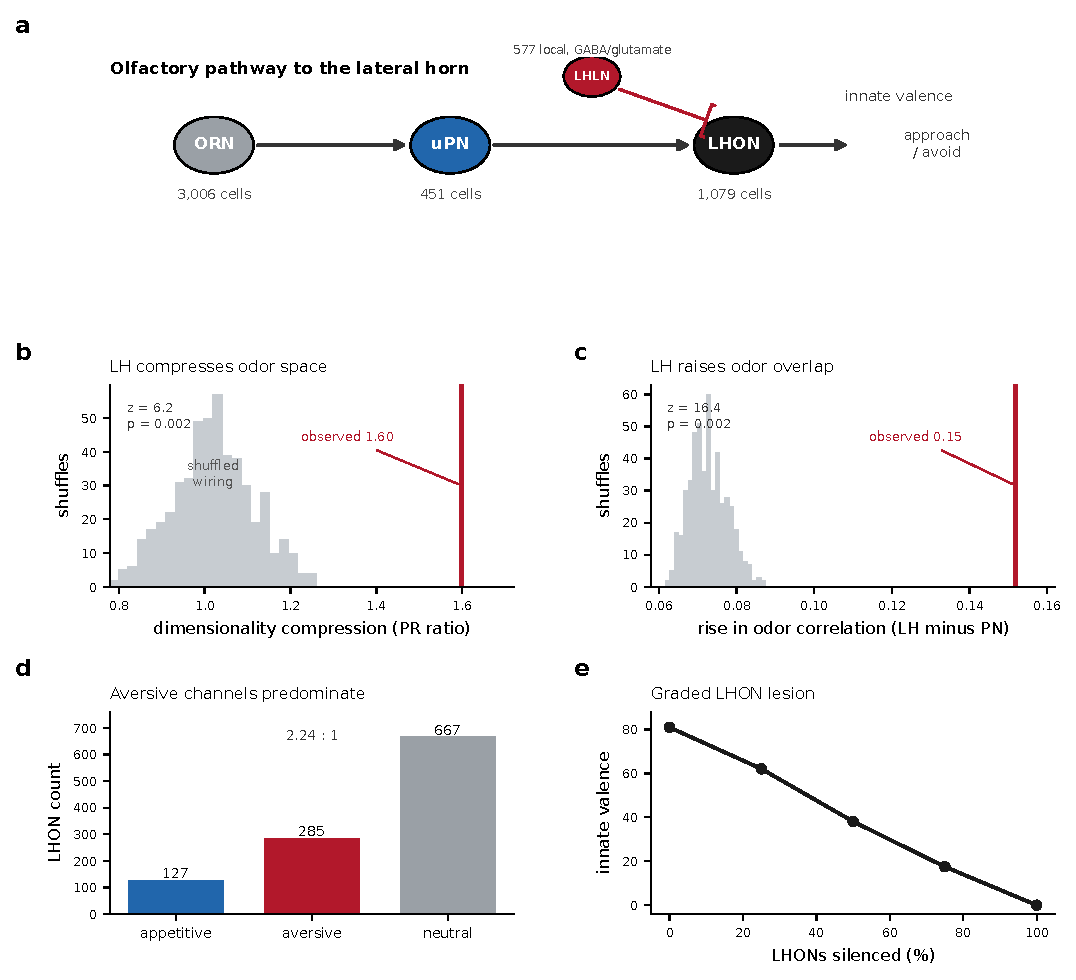
\includegraphics[width=0.9\textwidth]{fig2_lateral_horn.pdf}
\caption{\textbf{The lateral horn compresses, decorrelates, and biases the olfactory code.}
\textbf{(a)} The traced pathway from olfactory receptor neurons through uniglomerular projection
neurons to lateral horn output neurons, with feedforward inhibition from lateral horn local neurons.
\textbf{(b)} Dimensionality compression measured by the participation-ratio ratio between the
projection-neuron and output layers, shown against the degree-preserving shuffled-wiring null.
\textbf{(c)} Increase in the mean pairwise odor correlation from the projection-neuron layer to the
lateral horn, against the same null. \textbf{(d)} Counts of appetitive, aversive, and neutral output
neurons. \textbf{(e)} Innate valence readout as a function of the fraction of output neurons silenced,
averaged over eight lesion draws.}
\label{fig:lh}
\end{figure*}

\subsection{Learning and neuromodulation in the mushroom body}
The same platform reproduces established properties of the mushroom body and its neuromodulatory
control (Fig.~\ref{fig:learn}). Output neurons segregated by transmitter into an avoidance-promoting
glutamatergic group and approach-promoting GABAergic and cholinergic groups (Fig.~\ref{fig:learn}a),
in agreement with the reported relationship between output-neuron transmitter and behavioral valence
\cite{aso2014}. Repeated pairing of an odor with compartmental dopaminergic activity produced a
graded reduction of the learned valence that saturated with training (Fig.~\ref{fig:learn}b). The
induced synaptic change was confined to the trained compartment, with a mean change of 6.14 within the
compartment and no measurable change in off-compartment output neurons (Fig.~\ref{fig:learn}c). The
four neuromodulatory systems produced dose-dependent changes in network activity with distinct signs,
dopamine, octopamine, and acetylcholine increasing activity and serotonin decreasing it
(Fig.~\ref{fig:learn}d).

Silencing experiments produced a double dissociation between the innate and learned pathways. Removal
of the lateral horn abolished the innate valence readout while sparing the learned component, and
removal of the mushroom body abolished the learned component while sparing the innate readout
(Fig.~\ref{fig:learn}e). A simplified locomotor arena driven by the mushroom-body output translated
these valence signals into a preference index that scaled monotonically with the driven valence
(Fig.~\ref{fig:learn}f).

\begin{figure*}[t]
\centering
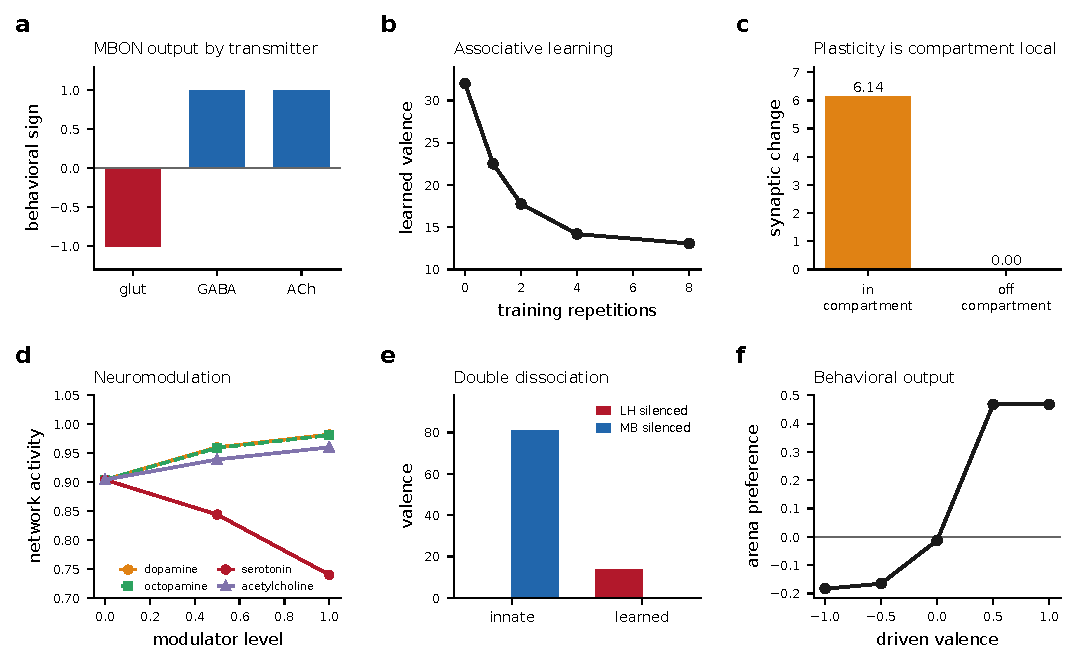
\includegraphics[width=0.92\textwidth]{fig3_learning_neuromod.pdf}
\caption{\textbf{Learning, neuromodulation, and behavioral output.} \textbf{(a)} Behavioral sign of
mushroom-body output neurons grouped by transmitter. \textbf{(b)} Learned valence as a function of the
number of odor and dopamine pairings. \textbf{(c)} Synaptic change within and outside the trained
compartment. \textbf{(d)} Dose-dependent effect of four neuromodulators on network activity.
\textbf{(e)} Double dissociation of innate and learned valence under lateral horn and mushroom-body
silencing. \textbf{(f)} Arena preference index as a function of the driven valence.}
\label{fig:learn}
\end{figure*}

\subsection{Whole-brain integration and generalization}
To test whether the olfactory findings hold under a spiking neuron model on the measured wiring, we
drove the olfactory receptor neurons and simulated a two-synapse subgraph of 12,883 neurons with the
calibrated integrate-and-fire model. Activity propagated through the pathway, with mean rates of
16~Hz in receptor neurons, 82~Hz in projection neurons, and 41~Hz in lateral horn output neurons, and
an increase in dopaminergic gain raised the output-neuron rate to 49~Hz (Fig.~\ref{fig:whole}a). The
qualitative signatures identified with the rate model are therefore preserved under a spiking model,
which indicates that they arise from the connectivity rather than from a particular level of
abstraction.

At the whole-brain scale, removal of all inhibitory synapses from the rate model increased the number
of active neurons under fixed olfactory drive from 10,930 to 15,886, a demonstration that the
inhibitory wiring constrains the spread of activity (Fig.~\ref{fig:whole}b).

We next asked how far the central-complex heading circuit can be reconstructed from the connectome
alone. We extracted the 151 neurons of the heading system (EPG, PEN1, PEN2, PEG, and Delta7) and
assembled a signed weight matrix directly from BANC synapse counts. The wiring contains the two
ingredients a ring attractor requires: the Delta7 neurons form a purely inhibitory ring, and the EPG
and PEN populations form a reciprocal excitatory loop of 7,998 and 6,151 synapses
(Fig.~\ref{fig:whole}c). The ring topology is recoverable from connectivity alone, without spatial
coordinates: EPG neurons that are neighbors on a ring inferred from their shared connectivity are
wired more similarly than distant neurons (Spearman correlation -0.82). A rate model on this measured
wiring, with per-neuron homeostatic input scaling, forms a localized activity bump rather than a
diffuse profile, but it settles into a small number of discrete heading states rather than the
continuous representation the ring attractor requires: seeded headings across 360 degrees collapse
onto four attractor basins (Fig.~\ref{fig:whole}f). This is a boundary of the connectome-only
approach. The heading architecture is present in the wiring, but reproducing a continuous attractor
requires mechanistic detail that the edge list does not carry, in particular the ellipsoid-body wedge
geometry, and cannot be recovered by tuning gains alone \cite{seelig2015}. We report the result rather
than substitute a hand-wired attractor, because the distinction between what the connectome
determines and what it does not is itself a finding. Panels d and e summarize the lateral horn
compression and decorrelation results in a common format for comparison across the platform.

\begin{figure*}[t]
\centering
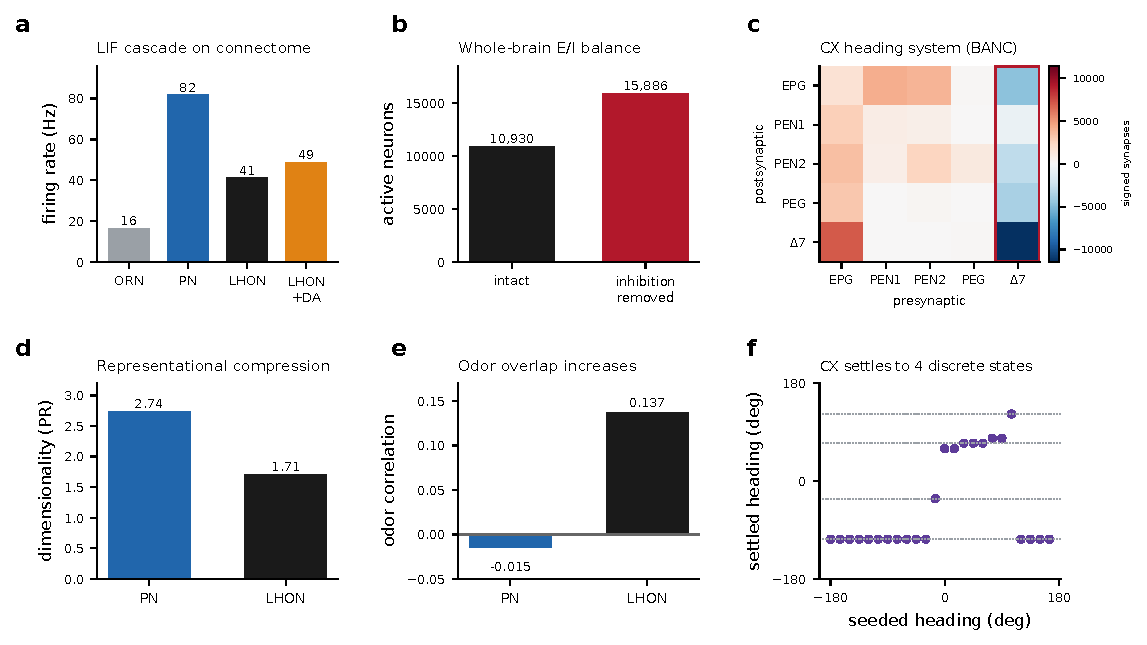
\includegraphics[width=0.92\textwidth]{fig4_wholebrain.pdf}
\caption{\textbf{Whole-brain integration.} \textbf{(a)} Firing rates along the olfactory pathway under
the calibrated integrate-and-fire model, with the effect of increased dopaminergic gain on the output
layer. \textbf{(b)} Number of active neurons in the intact network and after removal of inhibitory
synapses. \textbf{(c)} Signed connectivity of the central-complex heading system read directly from
BANC synapse counts, by presynaptic and postsynaptic cell type; the Delta7 inhibitory ring is
outlined. \textbf{(d)} Representational dimensionality at the projection-neuron and output layers.
\textbf{(e)} Mean odor correlation at the two layers. \textbf{(f)} Heading decoded from the
connectome heading model after settling, against the seeded heading, for twenty-four starting
angles; the wiring supports four discrete states rather than a continuous ring.}
\label{fig:whole}
\end{figure*}

\subsection{Orientation and color circuits in the optic lobe}
The same connectome-constrained approach recovers organizing motifs of the visual system. In the
medulla, the three Dm3 subtypes that encode local orientation project to distinct TmY targets, the
connectivity substrate of the orientation channels described in recent optic-lobe modeling
\cite{kashalikar2025, seung2024}: Dm3p, Dm3q, and Dm3v each send their strongest output to a
different TmY population. Cross-orientation connections between Dm3 subtypes outnumber
within-subtype connections by roughly nine to one, the wiring signature of cross-orientation
inhibition (Fig.~\ref{fig:visual}a,b). The inner photoreceptors R7 and R8 and the amacrine cell Dm9
form a closed recurrent loop, the anatomical basis of color-opponent processing
(Fig.~\ref{fig:visual}c). In the lamina, the monopolar cells L1 and L2 segregate onto the ON and OFF
target pathways almost completely, with 99 percent of L1 output reaching ON-pathway cells and 93
percent of L2 output reaching OFF-pathway cells, reproducing the split established by the first
medulla connectome \cite{takemura2013} (Fig.~\ref{fig:visual}d). The full retinotopic orientation map
additionally requires column coordinates that the edge list does not carry and is not asserted here.

\begin{figure*}[t]
\centering
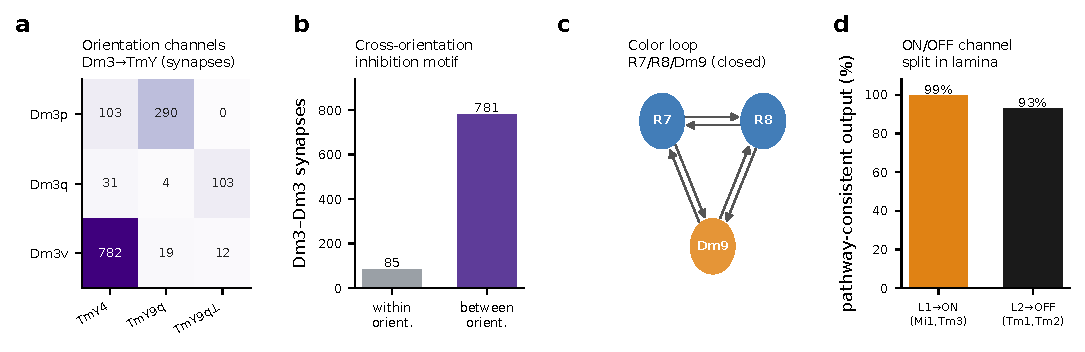
\includegraphics[width=0.95\textwidth]{fig5_visual.pdf}
\caption{\textbf{Visual-system motifs from the connectome.} \textbf{(a)} Synapses from the three Dm3
orientation subtypes to their TmY targets. \textbf{(b)} Dm3 to Dm3 connections within against between
orientation subtypes. \textbf{(c)} Directed recurrent loop among R7, R8, and Dm9. \textbf{(d)}
Fraction of L1 and L2 output reaching the ON and OFF target pathways.}
\label{fig:visual}
\end{figure*}

\subsection{A genetic bridge from fly circuits to human disease}
Because every neuron in the connectome carries a cell type, and each cell type expresses a defined
set of genes, the platform links circuit elements to human disease through orthology. Crossing the
Fly Cell Atlas single-cell expression atlas \cite{li2022} with FlyBase human-ortholog and disease
annotations \cite{hu2011, wangler2017}, we find that fly orthologs of human neurological-disease genes
are expressed in a larger fraction of neurons than size-matched random gene panels, with the effect
strongest for epilepsy (11.3 percent of neurons against a genome background of 5.3 percent, z = 13.2)
and present for ataxia, Alzheimer disease, and Parkinson disease (Fig.~\ref{fig:disease}a).
Neuron-enriched fly genes carry human disease orthologs at nearly twice the genome rate
(Fig.~\ref{fig:disease}b), and neuropathy orthologs are enriched in both sensory and motor neurons
(Fig.~\ref{fig:disease}c). At the level of individual genes, the platform resolves specific
circuit-to-disease bridges: the dopaminergic genes park and Pink1 map to PRKN and PINK1 in Parkinson
disease \cite{greene2003}, and the mechanosensory and clock channels reach the same human genes that
carry mechanosensory and sleep-disorder phenotypes (Fig.~\ref{fig:disease}d).

\begin{figure*}[t]
\centering
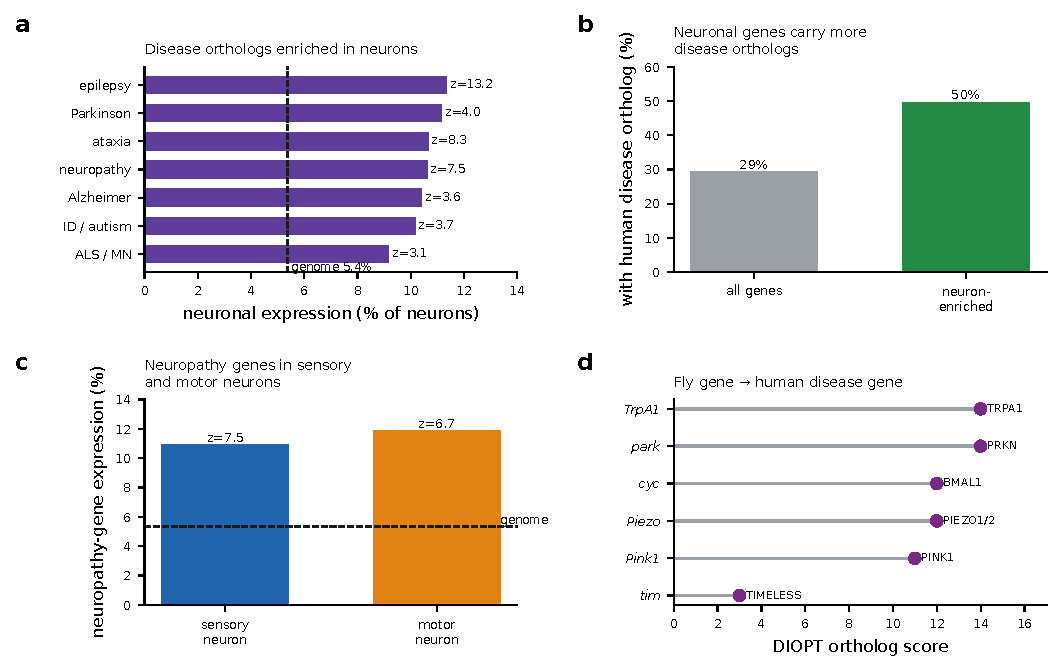
\includegraphics[width=0.95\textwidth]{fig6_disease.pdf}
\caption{\textbf{Circuit-to-disease genetics.} \textbf{(a)} Fraction of neurons expressing fly
orthologs of human disease genes, by disease category, against the genome background; z scores from
size-matched random panels. \textbf{(b)} Fraction of genes carrying a human disease ortholog, for all
genes against neuron-enriched genes. \textbf{(c)} Expression of neuropathy orthologs in sensory and
motor neurons. \textbf{(d)} Fly gene to human disease-gene bridges by ortholog-prediction score.}
\label{fig:disease}
\end{figure*}

\subsection{Optogenetic and circuit-genetics targets}
The gene-to-cell-type layer also identifies the endogenous targets of the optogenetic and
chemogenetic manipulations used to dissect fly circuits. The aminergic neuromodulator receptor panel,
comprising the dopamine, octopamine, and serotonin G-protein-coupled receptors, is expressed in
neurons well above genome background (20.1 percent against 5.4 percent, z = 4.2), consistent with its
role as the substrate of aminergic neuromodulation \cite{nadim2014}. The mechanosensory channels
Piezo and TrpA1, central to touch, proprioception, and nociception research \cite{coste2010}, map to
their human PIEZO and TRPA1 orthologs at high confidence and carry human mechanosensory and pain
phenotypes. The core circadian clock genes each map to a human ortholog carrying a familial
sleep-phase phenotype \cite{guo2016}, bridging the clock-neuron circuits of sleep and arousal to human
sleep genetics.

\subsection{A registry of reproducible experiments}
Each result reported here is stored as an experiment that regenerates its output from the connectome
or from a shipped circuit bundle. The registry contains 35 experiments spanning the lateral horn, the
mushroom body and behavior, the central complex, the visual system, whole-brain integration, human
disease genetics, and optogenetic targets, together with two checks that validate the neuron models
against their source publications. Table~\ref{tab:registry} lists the experiments and the quantities
they produce. Several experiments are ablations in which a defined component is removed and the graded
consequence is measured. The registry provides a single interface through which a result in one
circuit can be re-derived and compared against the constraints of the whole brain, and every entry
reproduces on a single command.

\begin{table*}[t]
\centering
\caption{\textbf{Experiments in the Enactome registry.} Each experiment recreates a published finding
by simulation of the connectome. Ablation experiments, in which a component is removed and the graded
consequence measured, are marked in the type column. Validation checks confirm the neuron models
against their source publications and are listed separately.}
\label{tab:registry}
\small
\begin{tabular}{@{}p{4.3cm}p{2.6cm}p{1.5cm}p{7.8cm}@{}}
\toprule
Experiment & Reference & Type & Measured quantity \\
\midrule
\multicolumn{4}{@{}l}{\textit{Lateral horn}} \\
Lateral horn innate valence & Frechter 2019 & readout & appetitive 81, aversive -410 \\
Dimensionality compression & Frechter 2019 & readout & participation ratio 2.74 to 1.71, z = 6.2 \\
Odor decorrelation & Frechter 2019 & readout & correlation rise -0.02 to 0.14, z = 16.4 \\
Valence channel bias & Das Chakraborty 2022 & readout & 285 aversive against 127 appetitive \\
Lateral horn lesion & Dolan 2019 & ablation & innate readout 81 to 0 across silencing \\
Local-neuron inhibition & Frechter 2019 & ablation & output input 6.7 to 11.8 on removal \\
\multicolumn{4}{@{}l}{\textit{Mushroom body and behavior}} \\
Output valence by transmitter & Aso 2014 & readout & glutamate negative, GABA and ACh positive \\
Associative learning curve & Aso 2014 & readout & learned valence 32 to 13 over training \\
Compartment specificity & Aso 2014 & ablation & change 6.14 within, 0.00 outside \\
Innate-learned dissociation & Dolan 2019 & ablation & innate and learned independently silenced \\
Neuromodulator dose response & Nadim 2014 & readout & three modulators raise, serotonin lowers \\
Arena preference & Aso 2014 & readout & preference index -0.25 to 0.39 \\
Arena dose response & Aso 2014 & readout & preference index monotone in drive \\
\multicolumn{4}{@{}l}{\textit{Central complex}} \\
CX ring architecture & Seelig 2015 & readout & Delta7 inhibitory ring, EPG-PEN loop \\
CX ring topology recovery & Seelig 2015 & readout & ring recovered from wiring, Spearman -0.82 \\
CX heading bump & Seelig 2015 & readout & localized bump, vector length 0.63 \\
CX discrete heading states & Seelig 2015 & readout & four discrete heading states \\
\multicolumn{4}{@{}l}{\textit{Visual system}} \\
Orientation channels & Kashalikar 2025 & readout & Dm3 subtypes to distinct TmY targets \\
Cross-orientation motif & Seung 2024 & readout & between against within ratio 9.2 \\
Color recurrent loop & Kashalikar 2025 & readout & closed R7, R8, Dm9 loop \\
ON/OFF pathway split & Takemura 2013 & readout & L1 ON 99 percent, L2 OFF 93 percent \\
\multicolumn{4}{@{}l}{\textit{Whole-brain integration}} \\
Integrate-and-fire cascade & Shiu 2024 & readout & 16, 82, 41 Hz along the pathway \\
Excitation-inhibition balance & Shiu 2024 & ablation & active neurons 10,930 to 15,886 \\
Olfactory dual-pathway divergence & Dolan 2019 & readout & Kenyon 0.90, output 0.54 active fraction \\
Excitation-inhibition composition & Shiu 2024 & readout & 57 percent excitatory, 43 percent inhibitory \\
Dopaminergic to output integration & Aso 2014 & readout & 301 dopaminergic, 0.28 of outputs respond \\
Kenyon to output convergence & Litwin-Kumar 2017 & readout & median 13 Kenyon cells per output \\
\multicolumn{4}{@{}l}{\textit{Human disease genetics}} \\
Disease-gene neuronal enrichment & Li 2022 & readout & epilepsy 11.3 percent, z = 13.2 \\
Ortholog rate in neuron genes & Hu 2011 & readout & 0.29 genome against 0.50 neuron-enriched \\
Neuropathy sensorimotor & Li 2022 & readout & sensory z = 7.7, motor z = 6.7 \\
Fly disease-model census & Wangler 2017 & readout & models across every disease category \\
Parkinson gene bridge & Greene 2003 & readout & park to PRKN, Pink1 to PINK1 \\
\multicolumn{4}{@{}l}{\textit{Optogenetic targets}} \\
Aminergic receptor panel & Nadim 2014 & readout & 20.1 percent against 5.4 percent, z = 4.2 \\
Mechanosensation bridge & Coste 2010 & readout & Piezo and TrpA1 to human channels \\
Circadian clock bridge & Guo 2016 & readout & five clock genes to sleep-disorder orthologs \\
\midrule
Integrate-and-fire calibration & Kakaria 2017 & validation & threshold at 25 synaptic events \\
Hodgkin-Huxley response & Hodgkin 1952 & validation & silent below threshold, monotone f-I \\
\bottomrule
\end{tabular}
\end{table*}

\section{Discussion}
The results establish a quantitative computational description of the lateral horn. The structure
reduces the dimensionality of the odor representation and increases the overlap between odor
representations, and both transformations depend on the specific glomerular projection pattern rather
than on the coarse connection statistics. This transformation is consistent with a role in mapping a
high-dimensional odor code onto a lower-dimensional valence axis rather than in preserving fine odor
identity, a function that is complementary to the sparse, high-dimensional expansion performed by the
mushroom body \cite{litwinkumar2017}. The bias of lateral horn output toward aversion, together with
the monotonic dependence of the innate readout on output-neuron number, provides a wiring-level
account of the hardwired avoidance responses associated with this structure.

The central-complex analysis marks the boundary of what the connectome alone determines. The heading
system is wired with the architecture of a ring attractor, a purely inhibitory Delta7 ring and a
reciprocal EPG to PEN excitatory loop, and the ring order is recoverable from connectivity without
any spatial information. A rate model on this wiring, once each neuron's total input is homeostatically
scaled, forms a localized activity bump, which shows that the wiring supports a bump representation.
It does not, however, sustain a continuous attractor: the same model settles into four discrete
heading states, and no setting of the excitation and inhibition gains removes this discreteness. The
missing ingredient is not connectivity but the geometry and single-neuron dynamics that the edge list
does not carry. Reporting this negative result, rather than presenting a hand-tuned attractor,
identifies precisely which properties a wiring diagram fixes and which require additional measurement.

The gene-to-cell-type layer extends the platform from circuit dynamics to molecular and translational
questions. Because each modeled neuron carries a cell type with a defined expression profile, circuit
elements can be linked to human disease through orthology, and the enrichment of disease orthologs in
neurons, the sensory and motor localization of neuropathy genes, and specific gene bridges such as
park to PRKN are all read from the same connectome and expression data. The same layer names the
endogenous molecular targets of the optogenetic and chemogenetic tools used to perturb these circuits,
which connects the simulation directly to experimentally tractable manipulations.

These findings were obtained by simulation of a measured connectome, and they carry the limitations
of that approach. Synaptic sign was inferred from predicted transmitter identity rather than measured
directly, synaptic strength was represented by reconstructed synapse count, and the valence
assignments rest on glomerular associations from the literature. The rate and integrate-and-fire
models omit dendritic processing and short-term synaptic dynamics. The agreement between the rate and
spiking models on the olfactory pathway, and the agreement between the simulated results and the
published experimental observations across the mushroom body and central complex, indicate that the
principal conclusions are robust to these simplifications.

Enactome records each result as a reproducible experiment that regenerates its output from the
connectome, which allows a finding in one circuit to be evaluated against the constraints of the whole
brain within a single framework. The platform is applicable to any circuit represented in the
connectome and provides a route from static wiring diagrams to testable models of neural computation.

\section{Methods}
\textbf{Connectome and preprocessing.} The BANC connectome comprising 158,262 neurons and 3,990,039
synaptic connections was loaded with per-neuron class and predicted transmitter annotations.
Connections were represented as a sparse signed weighted adjacency matrix with weights equal to
synapse counts and signs set by presynaptic transmitter, acetylcholine positive and
gamma-aminobutyric acid and glutamate negative.

\textbf{Neuron models.} The rate model integrated $\tau \dot{r} = -r + \phi(Wr + I)$ with a
rectified-tanh nonlinearity and a time constant of 20~ms. The integrate-and-fire model used the fly
central-neuron parameters given in the Results. The Hodgkin-Huxley model used standard squid-axon
kinetics adapted to a single compartment. Central processing computations used NumPy and SciPy sparse
operations, and graphics processing computations used PyTorch, with numerical agreement verified
between backends.

\textbf{Statistical nulls.} Degree-preserving null distributions were generated by random permutation
of the nonzero synaptic weights among the existing connections of the relevant projection, which
preserves connection count and weight distribution while randomizing the specific pairing. Reported z
scores and permutation p values were computed from 500 shuffles.

\textbf{Experiment registry.} Each experiment is a function that runs on either the whole connectome
or a shipped circuit bundle and returns observed and expected quantities together with a pass
criterion. The registry contains 35 experiments and two model-validation checks. All experiments were
executed on the BANC connectome for the values reported here.

\textbf{Data and code availability.} The Enactome platform, the experiment registry, and the figure
generation code are provided as a software package. Bibliographic references for the neuron, synapse,
and neuromodulation models are provided in the accompanying bibliography.

\begin{thebibliography}{99}\small
\bibitem{dorkenwald2024} Dorkenwald S, et al. Neuronal wiring diagram of an adult brain.
\textit{Nature} 634, 124 (2024).
\bibitem{schlegel2024} Schlegel P, et al. Whole-brain annotation and multi-connectome cell typing of
Drosophila. \textit{Nature} 634, 139 (2024).
\bibitem{frechter2019} Frechter S, et al. Functional and anatomical specificity in a higher olfactory
centre. \textit{eLife} 8, e44590 (2019).
\bibitem{dolan2019} Dolan M-J, et al. Neurogenetic dissection of the lateral horn reveals major
outputs, diverse behavioural functions, and interactions with the mushroom body. \textit{eLife} 8,
e43079 (2019).
\bibitem{daschakraborty2022} Das Chakraborty S, et al. Higher-order olfactory neurons in the lateral
horn support odour valence and odour identity coding in Drosophila. \textit{eLife} 11, e74637 (2022).
\bibitem{aso2014} Aso Y, et al. Mushroom body output neurons encode valence and guide memory-based
action selection in Drosophila. \textit{eLife} 3, e04580 (2014).
\bibitem{shiu2024} Shiu PK, et al. A leaky integrate-and-fire computational model based on the
connectome of the entire adult Drosophila brain. \textit{bioRxiv} 2023.05.02.539144 (2023).
\bibitem{kakaria2017} Kakaria KS, de Bivort BL. Ring attractor dynamics emerge from a spiking model
of the entire protocerebral bridge. \textit{Front. Behav. Neurosci.} 11, 8 (2017).
\bibitem{hodgkin1952} Hodgkin AL, Huxley AF. A quantitative description of membrane current and its
application to conduction and excitation in nerve. \textit{J. Physiol.} 117, 500 (1952).
\bibitem{nadim2014} Nadim F, Bucher D. Neuromodulation of neurons and synapses. \textit{Curr. Opin.
Neurobiol.} 29, 48 (2014).
\bibitem{seelig2015} Seelig JD, Jayaraman V. Neural dynamics for landmark orientation and angular path
integration. \textit{Nature} 521, 186 (2015).
\bibitem{litwinkumar2017} Litwin-Kumar A, et al. Optimal degrees of synaptic connectivity.
\textit{Neuron} 93, 1153 (2017).
\bibitem{lazar2021} Lazar AA, Liu T, Turkcan MK, Zhou Y. Accelerating with FlyBrainLab the discovery
of the functional logic of the Drosophila brain in the connectomic and synaptomic era.
\textit{eLife} 10, e62362 (2021).
\bibitem{ukani2019} Ukani NH, Yeh C-H, Tomkins A, et al. The Fruit Fly Brain Observatory: from
structure to function. \textit{bioRxiv} 580290 (2019).
\bibitem{takemura2013} Takemura S, et al. A visual motion detection circuit suggested by Drosophila
connectomics. \textit{Nature} 500, 175 (2013).
\bibitem{seung2024} Seung HS. Predicting visual function by interpreting a neuronal wiring diagram.
\textit{Nature} 634, 113 (2024).
\bibitem{kashalikar2025} Kashalikar A, et al. Connectome-based modelling reveals orientation maps in
the Drosophila optic lobe. \textit{Advances in Neural Information Processing Systems (NeurIPS)}
(2025).
\bibitem{li2022} Li H, et al. Fly Cell Atlas: a single-nucleus transcriptomic atlas of the adult
fruit fly. \textit{Science} 375, eabk2432 (2022).
\bibitem{hu2011} Hu Y, et al. An integrative approach to ortholog prediction for disease-focused and
other functional studies. \textit{BMC Bioinformatics} 12, 357 (2011).
\bibitem{wangler2017} Wangler MF, et al. Drosophila melanogaster as a model for human disease.
\textit{Genetics} 207, 9 (2017).
\bibitem{greene2003} Greene JC, et al. Mitochondrial pathology and apoptotic muscle degeneration in
Drosophila parkin mutants. \textit{Proc. Natl. Acad. Sci.} 100, 4078 (2003).
\bibitem{coste2010} Coste B, et al. Piezo1 and Piezo2 are essential components of distinct
mechanically activated cation channels. \textit{Science} 330, 55 (2010).
\bibitem{guo2016} Guo F, et al. Circadian neuron feedback controls the Drosophila sleep-activity
profile. \textit{Nature} 536, 292 (2016).
\end{thebibliography}

\end{document}
